\documentclass[11pt]{amsart}
\usepackage[a4paper,margin=1in]{geometry}
\usepackage{amssymb}
\usepackage{graphicx}
\usepackage{float}
\usepackage{tikz}
\usetikzlibrary{arrows.meta}
\usepackage[hidelinks]{hyperref}

\newtheorem{theorem}{Theorem}
\newtheorem{lemma}{Lemma}
\theoremstyle{remark}
\newtheorem*{remark}{Remark}
\DeclareMathOperator{\mex}{mex}

\definecolor{copyc}{RGB}{176,92,40}
\definecolor{inkmuted}{RGB}{85,85,85}

\title{A Mex Sequence That Is Not Ultimately Periodic}
\author{Vamshi Jandhyala}
\date{Preprint, version 1, 8 October 2026. Not peer reviewed.}
\subjclass[2020]{Primary 11B37; Secondary 11B13, 91A46}
\keywords{mex sequence, minimum excluded value, ultimately periodic, sum-free set, Sprague-Grundy, formal verification}

\begin{document}

\begin{abstract}
Start with a few nonnegative integers and keep appending the least nonnegative integer that is not a sum $a_i+a_{n-i}$ of two terms whose indices add up to the last index $n$ already written. Guy asked whether every such mex sequence is ultimately periodic. It is not: the sequence that starts $1,1,1,0,1,0,1,1$ is unbounded. The proof needs two facts. The zeros of the sequence sit at the positions with remainder $0$ or $3$ modulo $5$, and each zero copies an earlier value into the set whose least missing element is taken, so from the third block of five on, each block brings a value that no earlier block had. An appendix gives every term exactly. Both proofs are formally verified in Lean.
\end{abstract}

\maketitle

\noindent\emph{Status of this preprint.} Lemmas~\ref{lem:zeros} and~\ref{lem:twins}, Theorem~\ref{thm:main} and the exact values of Theorem~\ref{thm:exact} are formally verified in Lean~4 (Section~\ref{sec:lean}), using only Lean's standard axioms. Apart from the exact values, the remarks of Section~\ref{sec:remarks} are not formally verified, and this version has not yet been independently reviewed.

\section{Introduction}

Guy asked whether a simple rule for growing sequences, borrowed from the theory of games, always settles into a repeating pattern. Here is the rule, and a starting word for which it never does.
The least nonnegative integer missing from $\{0,1,3\}$ is $2$; the one missing from $\{1,2\}$ is $0$. This least missing number is called the \emph{mex}, short for \emph{minimum excluded value}, of the set.

Here is a way to grow a sequence with it. Start from $1,1,1,0,1,0,1,1$, numbered from position $0$ to position $7$. Pair the first term with the last, the second with the second-last, and so on. The pair sums are $1+1=2$, $1+1=2$, $1+0=1$ and $0+1=1$. The set of sums is $\{1,2\}$, whose mex is $0$, so append $0$ as the term at position $8$.

Repeat the same operation after each new term. More generally, start with nonnegative integers $a_0,a_1,\dots,a_k$. To find $a_{n+1}$, pair terms whose indices add up to $n$, the index of the last term already written, and take the mex of their sums:
\begin{equation}\label{eq:rule}
 a_{n+1}=\mex\{a_i+a_{n-i}:0\le i\le n\}\qquad(n\ge k).
\end{equation}
The left side is the new term; the right side takes the first missing number from all the pair sums. A sequence extended by this rule is a \emph{mex sequence}.

In Section~E27 of \emph{Unsolved Problems in Number Theory}, Guy asks whether mex sequences are ultimately periodic~\cite{Guy}. His example from $1,4,3,2$ continues
\[
 0,0,0,0,0,5,1,1,1,1,1,6,2,2,0,0,0,0,0,5,\dots
\]
and is periodic with period $14$ from its fourth term on (OEIS A067017~\cite{OEIS}). Are mex sequences always ultimately periodic, that is, periodic once finitely many terms are dropped?

The question comes from games. In the Sprague-Grundy theory of impartial games, the value of a position is the mex of the values of the positions reachable from it, and for octal games, where a move may split a heap in two, the value of a split position is a sum of two smaller values taken in base two without carries~\cite{WW}. Whether those value sequences are ultimately periodic is a long-standing open question, and Guy's mex sequences are a model of it with ordinary addition.

\begin{theorem}\label{thm:main}
The mex sequence that starts $1,1,1,0,1,0,1,1$ is unbounded. In particular it is not ultimately periodic.
\end{theorem}

The answer concerns Guy's question as he states it, with ordinary addition. The variant with addition without carries (OEIS A067018), which is the one closest to the games, is untouched by our argument.

Section~\ref{sec:look} looks at the data, and Section~\ref{sec:copy} explains the copying mechanism using one worked step. Section~\ref{sec:proof} proves Theorem~\ref{thm:main} from two lemmas, without computing the growing values. Section~\ref{sec:remarks} describes the exact values, the zeros and some open questions, and Section~\ref{sec:lean} the formal verification. Appendix~\ref{sec:exact} proves the exact values.

\section{A first look}\label{sec:look}

Written in rows of five, the first sixty terms of our sequence are
\[
\begin{array}{c|ccccc}
\text{block } b & a_{5b} & a_{5b+1} & a_{5b+2} & a_{5b+3} & a_{5b+4}\\ \hline
0 & 1 & 1 & 1 & 0 & 1\\
1 & 0 & 1 & 1 & 0 & 3\\
2 & 0 & 3 & 3 & 0 & 3\\
3 & 0 & 2 & 2 & 0 & 2\\
4 & 0 & 5 & 5 & 0 & 2\\
5 & 0 & 4 & 4 & 0 & 2\\
6 & 0 & 6 & 6 & 0 & 2\\
7 & 0 & 9 & 9 & 0 & 2\\
8 & 0 & 8 & 8 & 0 & 2\\
9 & 0 & 10 & 10 & 0 & 2\\
10 & 0 & 13 & 13 & 0 & 2\\
11 & 0 & 12 & 12 & 0 & 2
\end{array}
\]
After the first few rows, three patterns stand out. The first and fourth columns are zero. The last column is $2$. The second and third columns agree, and their common value keeps changing: $2,5,4$, then $6,9,8$, then $10,13,12$, each triple $4$ more than the one before. Figure~\ref{fig:seq} shows that the patterns persist for the first $150$ terms.

\begin{figure}[H]
\centering
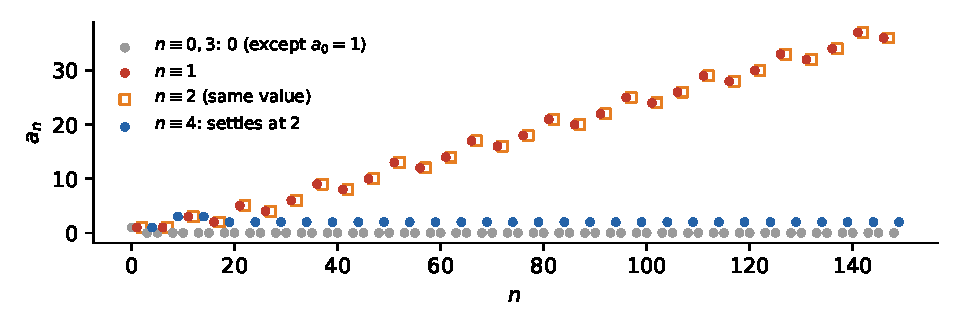
\includegraphics[width=0.8\textwidth]{figs/fig_sequence.pdf}
\caption{The first $150$ terms of the sequence started from $1,1,1,0,1,0,1,1$, coloured by the remainder of $n$ on division by $5$. Positions with remainder $0$ or $3$ hold $0$ (apart from $a_0=1$), positions with remainder $4$ settle at $2$, and the twin positions with remainders $1$ and $2$ carry equal values that grow by $4$ every three blocks.}
\label{fig:seq}
\end{figure}

To name the values, write $y_b=a_{5b+1}$ and $w_b=a_{5b+4}$. The data suggest that $a_{5b+2}=y_b$ too; we will prove that the two twin positions always agree. The table gives
\[
 y_0,y_1,\dots,y_7=1,1,3,2,5,4,6,9,\qquad w_0,w_1,\dots,w_7=1,3,3,2,2,2,2,2.
\]

\section{Why the values cannot settle}\label{sec:copy}

Before proving anything, here is the reason the twin values keep changing.

A zero is a copying device. If $a_j=0$, then the pair $(i,j)$ contributes $a_i+0=a_i$ to the set in~\eqref{eq:rule}: the value $a_i$ itself is excluded from being the next term. The data suggest that zeros sit at every position with remainder $0$ or $3$ on division by $5$, except position $0$. If this persists, they copy a great deal.

Take the term $a_{41}$, the first twin in block $8$. Its set uses the pairs $(i,40-i)$. Remainders add, and $40$ leaves remainder $0$, so a position with remainder $r$ is paired with one with remainder $5-r$ (or $0$ when $r=0$), and Figure~\ref{fig:pairs} shows what each pairing contributes. Two of the five pairings put a zero next to a twin position, so every twin value of an earlier block is copied into the set. Among the remaining pairs, a twin meets a position with remainder $4$, and two zeros meet. For example, positions $21$ and $19$ contribute $y_4+w_3=5+2=7$. In general for this step, a twin in block $c$ meets a remainder-$4$ value in block $7-c$, contributing $y_c+w_{7-c}$.

\begin{figure}[H]
\centering
\begin{tikzpicture}[x=1.9cm,y=1cm,
  box/.style={draw,minimum width=1.2cm,minimum height=0.75cm,font=\small},
  lab/.style={font=\scriptsize,fill=white,inner sep=1pt}]
\foreach \r/\v in {0/0,1/y,2/y,3/0,4/w} {
  \node[box] (t\r) at (\r,1.8) {$\v$};
  \node[font=\scriptsize,inkmuted,above] at (\r,2.2) {$i\equiv\r$};
}
\foreach \r/\v in {0/0,1/w,2/0,3/y,4/y} {
  \node[box] (b\r) at (\r,0) {$\v$};
}
\foreach \r/\s in {0/0,1/4,2/3,3/2,4/1} {
  \node[font=\scriptsize,inkmuted,below] at (\r,-0.4) {$40-i\equiv\s$};
}
\draw[inkmuted,thick] (t0.south)--(b0.north) node[lab,midway] {$0+0$};
\draw[inkmuted,thick] (t1.south)--(b1.north) node[lab,midway] {$y+w$};
\draw[copyc,very thick] (t2.south)--(b2.north) node[lab,midway,text=copyc] {$y+0=y$};
\draw[copyc,very thick] (t3.south)--(b3.north) node[lab,midway,text=copyc] {$0+y=y$};
\draw[inkmuted,thick] (t4.south)--(b4.north) node[lab,midway] {$w+y$};
\end{tikzpicture}
\caption{The pairs $(i,40-i)$ that determine $a_{41}$, grouped by remainders modulo $5$. The boxes show the usual values: $0$, a twin value $y$, or a last-column value $w$. In the first pairing there is one exception: position $0$ holds $1$, so $(0,40)$ and its reverse contribute $1$. The two highlighted pairings copy every earlier twin value.}
\label{fig:pairs}
\end{figure}

Collecting the contributions, the set for $a_{41}$ is $\{0,1,2,3,4,5,6,7,9,10\}$. Every earlier twin value, $1,2,3,4,5,6$ and $9$, is in it because a zero copied it, so the least missing value $a_{41}=8$ is new.

If this block pattern persists, the set for $a_{5b+1}$ contains every earlier twin value $y_0,\dots,y_{b-1}$, so the new value $y_b$ differs from all of them. Infinitely many distinct nonnegative integers cannot fit inside a bounded range. That would prove Theorem~\ref{thm:main}; we would not need to know the exact values of the twins. The remaining task is therefore to show that the zeros and twin positions persist. We do that next.

\section{The proof of unboundedness}\label{sec:proof}

The zeros have a useful independence: to decide whether a new term is zero, we need only know which earlier terms are zero. A pair sum is zero exactly when both terms are zero. If such a pair exists, the mex is positive; if none exists, the mex is zero.

For example, $a_9$ is positive because the zeros at positions $3$ and $5$ supply $0+0$ among its pair sums. But $a_{10}$ is zero: its pair indices add to $9$, which has remainder $4$ modulo $5$, and adding two zero-position remainders, $0$ or $3$, never gives remainder $4$. Figure~\ref{fig:zero-pattern} gives the whole remainder calculation.

\begin{figure}[H]
\centering
\begin{tikzpicture}[x=1cm,y=1cm,
 box/.style={draw,align=center,minimum width=3.1cm,minimum height=0.9cm,font=\small}]
\node[box] (z) at (0,0) {zero positions\\remainders $0,3$};
\node[box] (p) at (4.3,0) {zero-pair index sums\\remainders $0,1,3$};
\node[box] (n) at (8.6,0) {positive new terms\\remainders $1,2,4$};
\draw[-{Stealth[length=4pt]},inkmuted] (z.east)--(p.west) node[midway,above,font=\scriptsize] {add};
\draw[-{Stealth[length=4pt]},inkmuted] (p.east)--(n.west) node[midway,above,font=\scriptsize] {$+1$};
\node[font=\small,align=center] at (4.3,-1.1) {Missing pair-sum remainders $2,4$ give new zeros at remainders $3,0$.};
\end{tikzpicture}
\caption{How the zero pattern reproduces itself. All remainders are modulo $5$. The proof supplies actual zero pairs for the three possible sums, so the diagram describes positions as well as remainders. Position $0$, whose value is $1$, is excluded from the zero positions.}
\label{fig:zero-pattern}
\end{figure}

\begin{lemma}\label{lem:zeros}
Apart from $a_0=1$, the zeros occur exactly at positions with remainder $0$ or $3$ on division by $5$.
\end{lemma}

\begin{proof}
The starting eight terms have this pattern. Assume it holds before a new position $m\ge8$. Two zero positions can have index sum only with remainder $0$, $1$ or $3$, since their remainders are $0$ or $3$.

If $m$ has remainder $0$ or $3$, the pair indices must add to $m-1$, whose remainder is $4$ or $2$. No two zeros have such an index sum, so zero is missing from the pair sums and $a_m=0$.

For the other three remainders we must also check that a zero pair really exists, rather than just that its remainders are possible:
\[
\begin{array}{c|c|c}
m\bmod5 & \text{two zero positions} & \text{their sum}\\ \hline
1 & 5,\ m-6 & m-1\\
2 & 3,\ m-4 & m-1\\
4 & 3,\ m-4 & m-1
\end{array}
\]
In each row the two positions are positive, smaller than $m$, and have remainder $0$ or $3$. By induction they hold zeros. Thus zero is among the pair sums and $a_m>0$. This proves the pattern at every new position.
\end{proof}

Now the copying device from Section~\ref{sec:copy} is available at every block. The first two pairs of twins, at positions $1,2$ and $6,7$, are already equal in the starting word. We compare the sets used to choose the next two terms: the old twins and mixed sums stay the same, and the only extra contribution is larger than the first gap.

\begin{lemma}\label{lem:twins}
The two twin positions in every block agree: $a_{5b+1}=a_{5b+2}=y_b$. For each $b\ge2$, their value is at least $2$ and differs from every earlier twin value $y_0,\ldots,y_{b-1}$.
\end{lemma}

\begin{proof}
The starting word gives $y_0=y_1=1$. Assume the twins agree in every block before $b\ge2$, and let $T_b$ be the set of pair sums used to choose $a_{5b+1}$.

The pair indices add to $5b$, so the remainder pairs are $\{0,0\}$, $\{2,3\}$ and $\{1,4\}$, as in Figure~\ref{fig:pairs}. The first supplies $0$ from positions $5,5b-5$ and $1$ from positions $0,5b$. The second copies every old twin: positions $5c+2$ and $5(b-c)-2$ give $y_c+0$ for $0\le c<b$. The third supplies the mixed sums of an old twin with an old last-column value. Thus $T_b$ contains $0,1$ and every earlier twin. Its mex, $y_b=a_{5b+1}$, is at least $2$ and differs from all those twins.

For $a_{5b+2}$ the indices add to $5b+1$. The pair $\{0,1\}$ copies the same old twins, and $\{3,3\}$ supplies $0$. The mixed sums now come from $\{2,4\}$ instead of $\{1,4\}$: replacing an old first twin by its equal second twin increases the index sum by one without changing its value. These are exactly the same mixed sums. The boundary pair involving position $0$ now contributes $1+y_b$ instead of $1$, but $1=y_0$ is still among the copied twins. Therefore the new set is $T_b\cup\{1+y_b\}$.

The only added number is larger than the first gap $y_b$, so that gap remains the mex. Hence $a_{5b+2}=y_b$, completing the induction. Nothing here uses the sizes of the last-column values.
\end{proof}

\begin{proof}[Proof of Theorem~\ref{thm:main}]
Lemma~\ref{lem:twins} gives a new twin value different from every earlier one in each block $b\ge2$. Infinitely many distinct nonnegative integers cannot lie in a bounded range, so the sequence is unbounded. An ultimately periodic sequence has only finitely many different values, so this sequence is not ultimately periodic.
\end{proof}

\section{Remarks}\label{sec:remarks}

\emph{The exact values.} The proof of Theorem~\ref{thm:main} never uses the size of a twin value, only that it is new. The table suggests much more: after $1,1,3$ the twin values come in triples $2,5,4$, then $6,9,8$, and so on, each triple four more than the one before, and the last column is $2$ from block $3$ on. Theorem~\ref{thm:exact} in Appendix~\ref{sec:exact} proves this, so every term is known: for $n\ge15$, moving $15$ positions ahead adds $4$ at the twin positions and $0$ elsewhere.

\emph{The zeros of a mex sequence.} A pair sum is zero only when both terms are zero, so whether a new term is zero depends only on the earlier zero positions. Shifting every zero position up by one turns the rule into ordinary addition, since $(i+1)+(j+1)=(i+j+1)+1$. If $Y$ is the set of shifted zero positions of a mex sequence with starting word $a_0,\ldots,a_k$, then
\[
 y\in Y\quad\Longleftrightarrow\quad y\notin Y+Y\qquad(y\ge k+2),
\]
where $Y+Y=\{u+v:u,v\in Y\}$ allows $u=v$. This is the greedy completion of a sum-free set: starting from a finite set of positive integers containing no sum of two of its members, admit each larger integer exactly when it is not such a sum. Every greedy completion arises in this way. For a sum-free set with largest member $s$, take the word of length $s$ with a zero at position $u-1$ for each member $u$ and ones elsewhere; its shifted zero set is the greedy completion. (The starting set must be sum-free: the word $0,0$ gives the members $1,2$, and $2=1+1$.) Cameron asked whether every such completion is ultimately periodic, and Calkin and Finch list starting sets whose completions appear not to be, such as $\{1,3,8,20,26\}$~\cite{CF}. So even the zero positions of mex sequences lead to Cameron's question. In our example they are periodic after the initial term, and it is the other values that grow.

\emph{How the example was found.} We ran~\eqref{eq:rule} for every starting word of zeros and ones of length at most $8$, for $3000$ terms each. No word of length at most $7$ produced a value above $30$. Among the $256$ words of length $8$, exactly one produced a value above $100$: the word of Theorem~\ref{thm:main}, whose first $3000$ terms reach $797$.

\emph{Another example.} The first $4000$ terms of the sequence started from $1,1,0,0,1,1,0,1,0,1,1,1$ suggest another unbounded example. For every comparison available in that computation, $74\le n\le3951$, the difference $a_{n+48}-a_n$ is $7$ at $18$ fixed remainders modulo $48$ and $0$ at the other remainders. This is computational evidence; we have not proved that the pattern persists.

\emph{Open questions.} Our proved example has a repeating pattern of increments: from $n=15$ onward, moving $15$ positions ahead adds $4$ at the twin positions and $0$ elsewhere. The computations suggest a similar pattern for the second example. Call a sequence ultimately ``periodic plus linear'' when, after finitely many terms, $a_{n+p}-a_n$ depends only on the remainder of $n$ on division by some period $p$. Is every mex sequence ultimately of this form? Is there a mex sequence whose values grow faster than linearly, or one that is unbounded but returns to small values outside a periodic set of positions? And the question closest to the games remains open: is every mex sequence with addition without carries (OEIS A067018) ultimately periodic?

\section{Formal verification}\label{sec:lean}

The results of Section~\ref{sec:proof} and Appendix~\ref{sec:exact} are checked in the Lean~4 proof assistant (Lean 4.34 with Mathlib), in about $550$ lines that depend only on Lean's three standard axioms (propositional extensionality, choice and quotient soundness). A mex sequence is a function $a:\mathbb{N}\to\mathbb{N}$ with the starting word of Theorem~\ref{thm:main} that satisfies~\eqref{eq:rule} for every $n\ge7$.
\begin{itemize}
\item Lemmas~\ref{lem:zeros} and~\ref{lem:twins} and Theorem~\ref{thm:main} follow Section~\ref{sec:proof}, for any such sequence.
\item Lemma~\ref{lem:last} and Theorem~\ref{thm:exact} give every term, and with it a second proof of Theorem~\ref{thm:main}. Lean shows that this closed form satisfies~\eqref{eq:rule}, so that it is a mex sequence and the only one with this starting word. Positions below $60$ are checked by evaluation; beyond them the check is a symbolic case analysis on the residues of the positions, organised differently from the proof in Appendix~\ref{sec:exact}.
\end{itemize}
The Lean code, and a program that recomputes in exact arithmetic every number quoted in this paper, are at
\begin{center}\small\url{https://github.com/jvvk/mathematics/tree/main/mex-sequence-not-periodic}.\end{center}

\appendix

\section{The exact values}\label{sec:exact}

The zeros and twins suffice for unboundedness; the last column could have had any positive values. To find every term exactly, we first prove the additional pattern seen in the table: after $1,3,3$, the last-column values are all $2$.

\begin{lemma}\label{lem:last}
The last-column values are $w_0=1$, $w_1=w_2=3$, and $w_b=2$ for every $b\ge3$.
\end{lemma}

\begin{proof}
The first three values are in the table. Assume the claim for all last-column values before block $b\ge3$. To choose $a_{5b+4}$, the pair indices add to $5b+3$. The remainder pair $\{0,3\}$ supplies $0$ from positions $5,5b-2$ and $1$ from positions $0,5b+3$. The other pairs, $\{1,2\}$ and $\{4,4\}$, supply respectively
\[
 y_c+y_{b-c}\quad(0\le c\le b),\qquad
 w_c+w_{b-1-c}\quad(0\le c<b).
\]
These are sums of two twin values or two earlier last-column values. All are positive, so such a sum is $2$ only if both values are $1$. By Lemma~\ref{lem:twins}, only $y_0,y_1$ equal $1$; their block indices sum to at most $2$, rather than $b\ge3$. By the induction hypothesis, only $w_0$ equals $1$; its index cannot pair with itself to give $b-1\ge2$. Thus $2$ is missing while $0$ and $1$ are present, giving $w_b=2$ and completing the induction.
\end{proof}

We can now compute the first gap at the twin positions. Collecting the three kinds of sums in the proof of Lemma~\ref{lem:twins} gives, for $b\ge2$,
\begin{equation}\label{eq:twin-set}
 T_b=\{0,1\}\cup\{y_c:0\le c<b\}\cup\{y_c+w_{b-1-c}:0\le c<b\},\qquad y_b=\mex T_b.
\end{equation}
The set combines $0,1$, copies of all old twins, and mixed sums of an old twin with the last-column value in its paired block. The new twin is the first missing number. This is the general form of the worked computation for $a_{41}$ in Section~\ref{sec:copy}.

The table and the worked step give $y_0,\ldots,y_8=1,1,3,2,5,4,6,9,8$. For a first look at the next three blocks, equation~\eqref{eq:twin-set} gives
\[
 T_9=\{0,\ldots,9,12\},\qquad
 T_{10}=\{0,\ldots,12\},\qquad
 T_{11}=\{0,\ldots,11,13,14\}.
\]
Their first gaps are $10,13,12$, another copy of $2,5,4$ increased by $8$ (Figure~\ref{fig:three-gaps}).

\begin{figure}[H]
\centering
\begin{tikzpicture}[x=0.7cm,y=1cm]
\foreach \row/\b in {0/9,-1.4/10,-2.8/11} {
  \draw[inkmuted] (-0.3,\row)--(14.4,\row);
  \node[left,font=\small] at (-0.5,\row+0.25) {$T_{\b}$};
  \foreach \v in {0,...,14} {
    \draw[inkmuted] (\v,\row+0.05)--(\v,\row-0.05);
    \node[below,font=\scriptsize] at (\v,\row-0.05) {$\v$};
  }
}
\foreach \v in {0,...,9,12} \fill[inkmuted] (\v,0.25) circle (2.2pt);
\foreach \v in {0,...,12} \fill[inkmuted] (\v,-1.15) circle (2.2pt);
\foreach \v in {0,...,11,13,14} \fill[inkmuted] (\v,-2.55) circle (2.2pt);
\foreach \gap/\row in {10/0,13/-1.4,12/-2.8} {
  \draw[copyc,thick] (\gap,\row+0.25) circle (3.5pt);
  \node[above,font=\scriptsize,text=copyc] at (\gap,\row+0.35) {first gap};
}
\end{tikzpicture}
\caption{The first gap moves through $10,13,12$ in three consecutive blocks. Filled dots are numbers present in the set; the open circle is its mex. The proof below explains why the same pattern returns four units farther along.}
\label{fig:three-gaps}
\end{figure}

\begin{theorem}\label{thm:exact}
The twin values in blocks $0,1,2$ are $1,1,3$. Thereafter they come in triples $2,5,4$, then $6,9,8$, and so on, each triple four more than the previous one. Equivalently,
\[
 y_{3k+3}=4k+2,\qquad y_{3k+4}=4k+5,\qquad y_{3k+5}=4k+4\qquad(k\ge0).
\]
Together with the zero positions in Lemma~\ref{lem:zeros} and the last-column values in Lemma~\ref{lem:last}, this specifies every term of the sequence.
\end{theorem}

\begin{proof}
The table and the worked step verify the formula through block $8$. Assume it holds for all twin values before block $b\ge9$. In~\eqref{eq:twin-set}, the last-column value is usually $2$; only the last three mixed sums use the early values $w_2=3$, $w_1=3$, $w_0=1$. Thus
\begin{equation}\label{eq:twin-expanded}
 T_b=\{0,1\}\cup\{y_c:0\le c<b\}\cup\{y_c+2:0\le c\le b-4\}
       \cup\{y_{b-3}+3,y_{b-2}+3,y_{b-1}+1\}.
\end{equation}
In words, we have the old twins, copies of the sufficiently old twins moved two places to the right, and three exceptional contributions from the last three old blocks. For the numerical examples above, every number $0$ through $8$ is present; the contributions at $9$ or above are
\[
\begin{array}{c|c|c|c|c}
 b & \text{old twins} & \text{old twins}+2 & \text{three exceptions} & \text{first gap}\\ \hline
 9 & 9 & \text{none} & 9,12,9 & 10\\
 10 & 9,10 & \text{none} & 12,11,11 & 13\\
 11 & 9,10,13 & 11 & 11,13,14 & 12
\end{array}
\]
We now make the same count for any three-block group. Write $b=3k+3+r$, where $r=0,1,2$ says whether $b$ is the first, second or third block in its group. Here $k\ge2$ because $b\ge9$.

\emph{Fill the numbers below the current group.} The earlier triples $4k'+2,4k'+5,4k'+4$ with $0\le k'<k$ supply every number from $2$ to $4k+1$ except $3,7,11,\ldots,4k-1$. The value $3=y_2$ is itself an old twin. Each later hole is two more than an old twin: $4k'+7=(4k'+5)+2$. Its twin has block index $c=3k'+4\le3k-2\le b-4$, so the shifted copy is allowed in~\eqref{eq:twin-expanded}. With $0,1$, this fills every number through $4k+1$.

\emph{Locate the first gap above that filled interval.} The three possibilities are exactly those in the numerical table.
\begin{itemize}
\item First block ($r=0$). The candidate $4k+2$ is not an old twin. A shifted copy could reach it only from $4k$, whose block is $b-1$ and is too recent. The three exceptions are $4k+1,4k+4,4k+1$, so none fills it. The first gap is $4k+2$.
\item Second block ($r=1$). The previous block supplies $4k+2$; the exceptions $4k+4,4k+3,4k+3$ fill the next two places. But $4k+5$ is not an old twin, and a shifted copy could reach it only from $4k+3$. No twin has that value: past the initial values, twins never have remainder $3$ modulo $4$. The exceptions do not fill it either. The first gap is $4k+5$.
\item Third block ($r=2$). The old twins include $4k+2$ and $4k+5$. A shifted copy fills $4k+3$: its source is $y_{3k+1}=4k+1$, whose block index is $b-4$. The candidate $4k+4$ is not an old twin. Its only possible shifted source, $4k+2$, is in block $b-2$ and is too recent. The exceptions are $4k+3,4k+5,4k+6$, so the first gap is $4k+4$.
\end{itemize}
The initial twins $1,1,3$, shifted by $2$, give at most $5$, below all these candidates. The three gaps therefore prove the claimed formulas and complete the induction.
\end{proof}

\section*{Acknowledgement}

The proofs, text, verification programs and Lean formalisation were developed with the AI assistants Claude (Anthropic) and Codex (OpenAI), under the author's direction. The author is responsible for the contents.

{\small
\begin{thebibliography}{9}
\bibitem{WW} E.~R.~Berlekamp, J.~H.~Conway and R.~K.~Guy, \emph{Winning Ways for Your Mathematical Plays}, Academic Press, London, 1982.
\bibitem{CF} N.~J.~Calkin and S.~R.~Finch, Conditions on periodicity for sum-free sets, \emph{Experiment.\ Math.} \textbf{5} (1996), no.~2, 131--137, \href{https://doi.org/10.1080/10586458.1996.10504584}{doi:10.1080/10586458.1996.10504584}.
\bibitem{Guy} R.~K.~Guy, \emph{Unsolved Problems in Number Theory}, 3rd ed., Problem Books in Mathematics, Springer, New York, 2004, Section E27, pp.~349--350, \href{https://doi.org/10.1007/978-0-387-26677-0}{doi:10.1007/978-0-387-26677-0}.
\bibitem{OEIS} OEIS Foundation, \emph{The On-Line Encyclopedia of Integer Sequences}, sequences A067016, A067017 and A067018, \url{https://oeis.org}, accessed 8 October 2026.
\end{thebibliography}
}

\end{document}
